% !TEX TS-program = xelatex
% !TEX encoding = UTF-8 Unicode
% !Mode:: "TeX:UTF-8"

\documentclass[10pt]{resume}
\usepackage{graphicx}
\usepackage{tabu}
\usepackage{multirow}
\usepackage{progressbar}
%% Simplified Chinese Support using external fonts (./fonts/zh_CN-Adobe/)
\usepackage{zh_CN-Adobefonts_external}

\usepackage{linespacing_fix} % disable extra space before next section
\usepackage{cite}
\usepackage{setspace}
\begin{document}
\pagenumbering{gobble} % suppress displaying page number

\Large{
  \begin{tabu}{ c l r }
    \multirow{4}{1in}{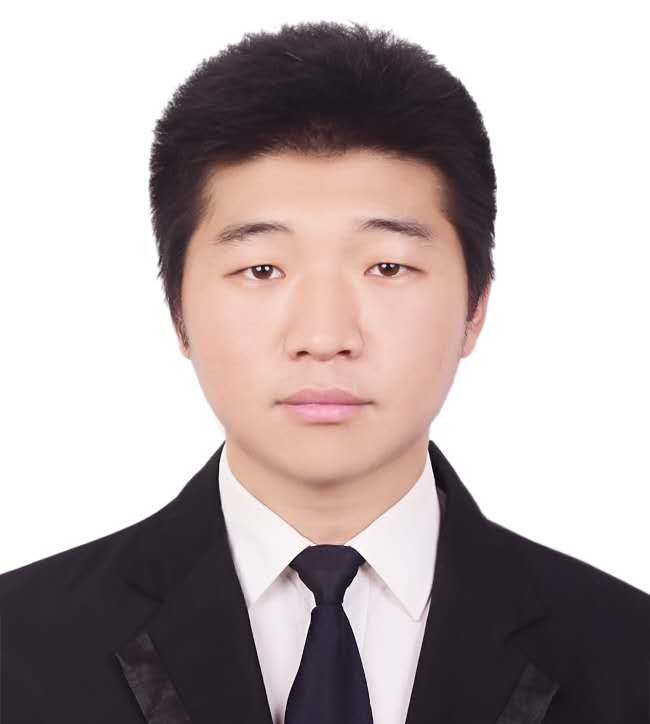
\includegraphics[width=1in]{profile}} & \scshape{高亚虎} & {Linux~}\progressbar{0.55} \\
    & \email{gao\_yahu@163.com} & {Python~}\progressbar{0.50} \\
    & \phone{(+86) 131-2029-0626\ \ \ \ } & {C~}\progressbar{0.5} \\
    & \github[github.com/yahugao]{https://github.com/yahugao} & {shell~}\progressbar{0.3}
  \end{tabu}
}

\section{\faGraduationCap\ 知识与技能}\normalsize
\begin{itemize}
  \item {熟悉常用的文本向量化方法BOW、TF-IDF,词向量方法one-hot、word2vec、ELMo和Bert.}
  \item {有FastText、TextCNN、BiLSTM、HAN等深度学习模型以及的传统机器学习算法LR、SVM、DT使用经验。}
%%  \item {了解深度学习中的网络结构设计方法以及其中的正则化和优化方法, 对常用的循环神经网络和卷积网络的基本结构有初步认识。}
  \item {有keras、TensorFlow和Pytorch的使用经验; 能熟练使用版本控制工具Git; 熟悉Linux内核。}
  \end{itemize}

\section{\faCogs\ 项目经验}\normalsize
%% \datedsubsection{\textbf{智能问答系统}, FlyAI竞赛平台}{2020年07月15日 -- 2020年09月08日}
%% 检索式问答系统,基于tf-idf对句子进行相似度计算, 从已有的问答对中取出和用户问题最相近的问题和答案
%% \datedsubsection{\textbf{知识图谱}, 阿里云天池竞赛平台}{2020年07月15日 -- 2020年09月08日}
\datedsubsection{\textbf{中医药说明书实体识别}, 阿里云天池竞赛平台}{2020年09月10日 -- 今天}
\begin{itemize}
\item{竞赛项目。基于已有的中医药说明书和其对应的实体标注,训练模型对其它中医药说明书中出现的相关实体进行预测。共有13类实体,采用BIO标注方法对文本中的token进行处理,将其转化为分类问题。借助bert预训练词向量,对说明书中的文本进行向量化表示,结合CRF对药品说明书中的token所属的类别进行预测。以F1-score为衡量标准,目前在线得分为0.7496.}
\end{itemize}
\datedsubsection{\textbf{新闻文本分类}, 阿里云天池竞赛平台}{2020年08月17日 -- 2020年09月08日}
\begin{itemize}
\item{竞赛项目。数据进行字符匿名处理的新闻数据,共有14个类别,20W样本,测试集为2W条样本。基于文本内容预测新闻所属的类别。分别使用机器学习的SVM、Naive Bayes和深度学习的FastText、CNN、RNN、RCNN和HAN对训练集进行了特征抽取和类别预测。以F1-score为衡量标准,SVM的效果最好达到了0.924; 深度学习方法中,对HAN模型进行添加卷积层、使用动态学习率、早停、改变词嵌入维度、向其中的LSTM添加dropout并调整输出维度的优化后,f1-score最终得分为0.896.}
\end{itemize}
\datedsubsection{\textbf{微博立场检测}, FlyAI竞赛平台}{2020年03月15日 -- 2020年05月6日}
 \begin{itemize}
 \item {竞赛项目。借助已有的微博预训练词向量,使用Pytorch构建双向LSTM网络,对微博中表现的立场进行检测。模型使用f1-score进行评测,经过数据清洗,超参数调整,使用变长序列,早停和dropout等优化方法后,模型的得分由0.27提升到了0.53.}
 \end{itemize}
\section{\faUsers\ 个人经历}\normalsize
\datedsubsection{\textbf{瞬联软件科技有限公司}\ Linux系统工程师}{2017年09月 -- 2019年11月}
\begin{itemize}
\item {参与WindRiver Linux系统的研发与测试,负责调查和维护系统新版本发布和运行中出现的问题。涉及toolchain、Linux Kernel和用户态软件的漏洞监控和修复以及内核crash的debug。在bug无法复现时有能力结合堆栈信息和内核源码定位并修复问题; 对系统中涉及的CVE漏洞进行监控和修复。曾根据堆栈信息, 修复了三周复现一次的Procfs 引起的内核crash。为团队搭建了git仓库管理系统。因妻子需要出国访学一年,辞职陪读,现已回国。}
\end{itemize}
% \section{\faUsers\ 实习经历}
\datedsubsection{\textbf{英特尔(中国)有限公司}\ 实习软件工程师}{2016年8月 -- 2017年2月}
\begin{itemize}
\item {完成了LTP(Linux test project)由PC端向移动端的移植与验证,解决了LTP在平台迁移过程中的不兼容问题, 向LTP开源社区成功提交了修复数据类型的patch。}
\end{itemize}
% \section{\faGraduationCap\  教育背景}
\datedsubsection{\textbf{中国人民解放军信息工程大学}\ 硕士研究生:\ 计算机科学与技术}{2014年9月 -- 2017年7月}
\begin{itemize}
\item {研究方向为软件分析与逆向工程,期间发表学术论文两篇(知网检索一篇), 学位论文一篇。}
\end{itemize}
\datedsubsection{\textbf{河北理工大学(现华北理工大学)}\ 本科:\ 计算机科学与技术}{2010年9月 -- 2014年7月}
%% \vspace{1ex}
\section{\faInfo\ 其他}
% increase linespacing [parsep=0.5ex]
\begin{itemize}\normalsize
\item {两年的bug修复经验,养成了工作认真,思维严谨的好习惯。自学机器学习和自然语言处理,具有良好的自我驱动学习能力。喜欢健身、跑步,身体健康。}
  \end{itemize}

\end{document}

%%% Local Variables:
%%% mode: latex
%%% TeX-master: t
%%% End:
